\documentclass[tikz,border=5pt]{standalone}
\usepackage{amssymb,amsmath}
\newcommand{\C}{\mathbb{C}}
\newcommand{\CP}{\mathbb{CP}}
\newcommand{\Res}{\operatorname{Res}}
\begin{document}
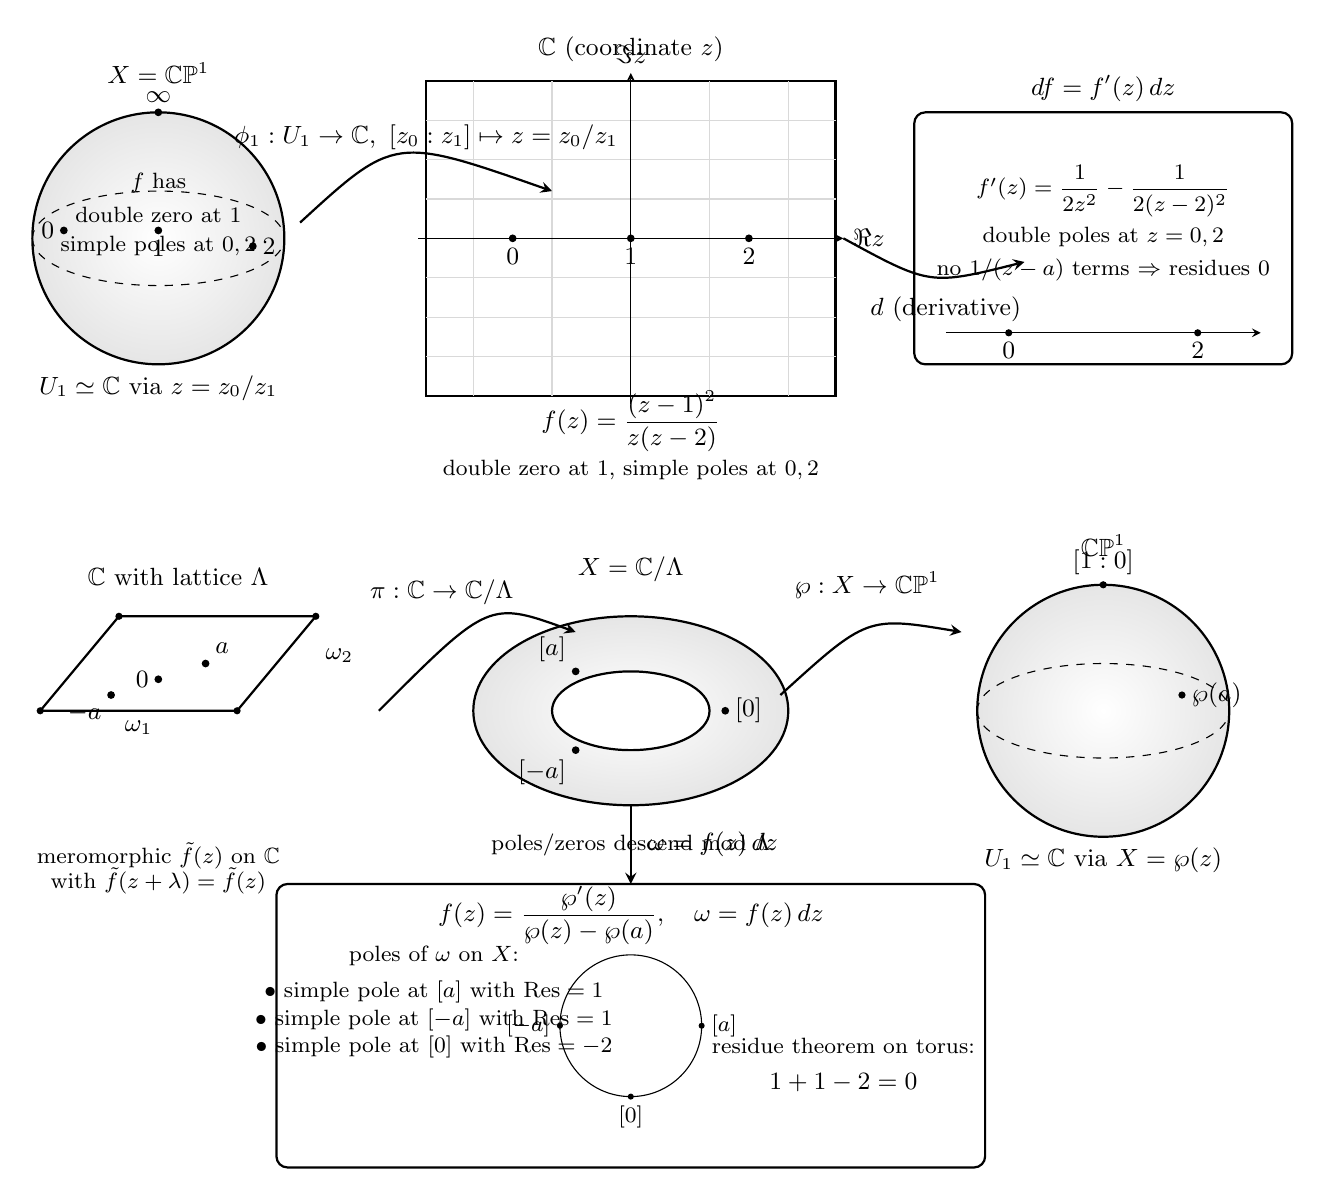
\begin{tikzpicture}[font=\small,>=stealth]
	
	%====================================================
	% TOP ROW: X = CP^1, f(z) and df
	%====================================================
	
	%-------------------------
	% (1) CP^1 as Riemann sphere
	%-------------------------
	\begin{scope}[shift={(-6,3)}]
		% Sphere
		\shade[inner color=white, outer color=gray!20, draw=black, thick]
		(0,0) circle (1.6);
		\node at (0,2.1) {$X=\CP^1$};
		
		% North pole: infinity
		\fill (0,1.6) circle (1.4pt);
		\node[above] at (0,1.6) {$\infty$};
		
		% Equator = U_1
		\draw[dashed] (-1.6,0) arc (180:360:1.6 and 0.6);
		\draw[dashed] (-1.6,0) arc (180:0:1.6 and 0.6);
		\node at (0,-1.9) {$U_1\simeq\C$ via $z=z_0/z_1$};
		
		% Mark finite points 0,1,2 on equator
		\fill (-1.2,0.1) circle (1.4pt);
		\node[left] at (-1.2,0.1) {$0$};
		\fill (0,0.1) circle (1.4pt);
		\node[below] at (0,0.1) {$1$};
		\fill (1.2,-0.1) circle (1.4pt);
		\node[right] at (1.2,-0.1) {$2$};
		
		% Labels for zero/pole structure of f
		\node at (0,0.7) {\footnotesize $f$ has};
		\node at (0,0.3) {\footnotesize double zero at $1$};
		\node at (0,-0.1) {\footnotesize simple poles at $0,2$};
	\end{scope}
	
	%-------------------------
	% (2) z-plane (affine chart)
	%-------------------------
	\begin{scope}[shift={(0,3)}]
		% Rectangle for C
		\draw[thick] (-2.6,-2.0) rectangle (2.6,2.0);
		\node at (0,2.4) {$\C$ (coordinate $z$)};
		
		% Grid
		\foreach \x in {-2,-1,...,2}
		\draw[gray!30] (\x,-2.0) -- (\x,2.0);
		\foreach \y in {-1.5,-1,...,1.5}
		\draw[gray!30] (-2.6,\y) -- (2.6,\y);
		
		% Axes
		\draw[->] (-2.7,0) -- (2.7,0) node[right] {$\Re z$};
		\draw[->] (0,-2.1) -- (0,2.1) node[above] {$\Im z$};
		
		% Points 0,1,2
		\fill (-1.5,0) circle (1.4pt) node[below] {$0$};
		\fill (0,0) circle (1.4pt) node[below] {$1$};
		\fill (1.5,0) circle (1.4pt) node[below] {$2$};
		
		% Label for f
		\node[align=center] at (0,-2.5)
		{$f(z)=\dfrac{(z-1)^2}{z(z-2)}$\\[2pt]
			\footnotesize double zero at $1$, simple poles at $0,2$};
		
	\end{scope}
	
	% Arrow: CP^1 (U1) -> C (chart z)
	\draw[->,thick]
	(-4.2,3.2) .. controls (-3,4.3) .. (-1.0,3.6);
	\node[above] at (-2.6,4.0) {$\phi_1:U_1\to\C,\ [z_0:z_1]\mapsto z=z_0/z_1$};
	
	%-------------------------
	% (3) 1-form df = f'(z) dz
	%-------------------------
	\begin{scope}[shift={(6,3)}]
		% Small box for "world of 1-forms"
		\draw[thick,rounded corners] (-2.4,-1.6) rectangle (2.4,1.6);
		\node at (0,1.9) {$df = f'(z)\,dz$};
		
		% Show pole structure of df
		\node[align=center] at (0,0.6)
		{\footnotesize $f'(z)=\dfrac{1}{2z^2}-\dfrac{1}{2(z-2)^2}$};
		\node[align=center] at (0,-0.2)
		{\footnotesize double poles at $z=0,2$\\[1pt]
			\footnotesize no $1/(z-a)$ terms $\Rightarrow$ residues $0$};
		
		% Small sketch: z-axis with 0 and 2
		\draw[->] (-2.0,-1.2) -- (2.0,-1.2);
		\fill (-1.2,-1.2) circle (1.3pt) node[below] {$0$};
		\fill (1.2,-1.2) circle (1.3pt) node[below] {$2$};
	\end{scope}
	
	% Arrow: f on C -> df box
	\draw[->,thick]
	(2.7,3.0) .. controls (3.8,2.4) .. (5.0,2.7);
	\node at (4.0,2.1) {$d$ (derivative)};
	
	%====================================================
	% BOTTOM ROW: X = C / Λ, wp, wp', elliptic f, residues
	%====================================================
	
	%-------------------------
	% (4) Lattice in C (covering of torus)
	%-------------------------
	\begin{scope}[shift={(-6,-3)}]
		% Fundamental parallelogram
		\draw[thick] (-1.5,0) -- (1.0,0) -- (2.0,1.2) -- (-0.5,1.2) -- cycle;
		\node at (0.25,1.7) {$\C$ with lattice $\Lambda$};
		
		% Label edges as periods
		\node[below] at (-0.25,0) {$\omega_1$};
		\node[right] at (2.0,0.7) {$\omega_2$};
		
		% Some lattice points (dots)
		\foreach \x/\y in {-1.5/0, 1.0/0, -0.5/1.2, 2.0/1.2}
		\fill (\x,\y) circle (1.3pt);
		
		% Mark 0 and ±a
		\fill (0.0,0.4) circle (1.4pt);
		\node[left] at (0.0,0.4) {$0$};
		
		\fill (0.6,0.6) circle (1.4pt);
		\node[above right] at (0.6,0.6) {$a$};
		
		\fill (-0.6,0.2) circle (1.4pt);
		\node[below left] at (-0.6,0.2) {$-a$};
		
		\node[align=center] at (0,-2.0)
		{\footnotesize meromorphic $\tilde f(z)$ on $\C$\\[-2pt]
			\footnotesize with $\tilde f(z+\lambda)=\tilde f(z)$};
	\end{scope}
	
	%-------------------------
	% (5) Torus X = C / Λ
	%-------------------------
	\begin{scope}[shift={(0,-3)}]
		% Torus as donut
		\shade[inner color=white, outer color=gray!20, draw=black, thick]
		(0,0) ellipse (2.0 and 1.2);
		\fill[white] (0,0) ellipse (1.0 and 0.5);
		\draw[black,thick] (0,0) ellipse (1.0 and 0.5);
		\node at (0,1.8) {$X=\C/\Lambda$};
		
		% Mark [0], [a], [-a]
		\fill (1.2,0) circle (1.4pt);
		\node[right] at (1.2,0) {$[0]$};
		
		\fill (-0.7,0.5) circle (1.4pt);
		\node[above left] at (-0.7,0.5) {$[a]$};
		
		\fill (-0.7,-0.5) circle (1.4pt);
		\node[below left] at (-0.7,-0.5) {$[-a]$};
		
		% Small label
		\node at (0,-1.7) {\footnotesize poles/zeros descend mod $\Lambda$};
	\end{scope}
	
	% Arrow: C -> torus (quotient)
	\draw[->,thick]
	(-3.2,-3.0) .. controls (-1.8,-1.6) .. (-0.7,-2.0);
	\node at (-2.4,-1.5) {$\pi:\C\to\C/\Lambda$};
	
	%-------------------------
	% (6) CP^1 target with wp, wp'
	%-------------------------
	\begin{scope}[shift={(6,-3)}]
		% Sphere
		\shade[inner color=white, outer color=gray!20, draw=black, thick]
		(0,0) circle (1.6);
		\node at (0,2.1) {$\CP^1$};
		
		% North pole = infinity
		\fill (0,1.6) circle (1.3pt);
		\node[above] at (0,1.6) {$[1:0]$};
		
		% Equator = affine chart for wp
		\draw[dashed] (-1.6,0) arc (180:360:1.6 and 0.6);
		\draw[dashed] (-1.6,0) arc (180:0:1.6 and 0.6);
		\node at (0,-1.9) {$U_1\simeq\C$ via $X=\wp(z)$};
		
		% Mark typical values
		\fill (1.0,0.2) circle (1.3pt);
		\node[right] at (1.0,0.2) {$\wp(a)$};
	\end{scope}
	
	% Arrow: torus -> CP^1 (wp)
	\draw[->,thick]
	(1.9,-2.8) .. controls (3.0,-1.8) .. (4.2,-2.0);
	\node at (3.0,-1.4) {$\wp:X\to\CP^1$};
	
	%-------------------------
	% (7) Box for elliptic function f(z) dz and residues
	%-------------------------
	\begin{scope}[shift={(0,-7.0)}]
		\draw[thick,rounded corners] (-4.5,-1.8) rectangle (4.5,1.8);
		\node at (0,1.4)
		{$f(z) = \dfrac{\wp'(z)}{\wp(z)-\wp(a)},\quad \omega = f(z)\,dz$};
		
		% Poles and residues
		\node[align=center] at (-2.5,0.3)
		{\footnotesize poles of $\omega$ on $X$:\\[2pt]
			\footnotesize $\bullet$ simple pole at $[a]$ with $\Res=1$\\[-1pt]
			\footnotesize $\bullet$ simple pole at $[-a]$ with $\Res=1$\\[-1pt]
			\footnotesize $\bullet$ simple pole at $[0]$ with $\Res=-2$};
		
		\node[align=center] at (2.7,-0.5)
		{\footnotesize residue theorem on torus:\\[2pt]
			$1 + 1 - 2 = 0$};
		
		% Little sketch: [a],[-a],[0] on a circle
		\draw (0,0) circle (0.9);
		\fill (0.9,0) circle (1.1pt) node[right] {\footnotesize $[a]$};
		\fill (-0.9,0) circle (1.1pt) node[left] {\footnotesize $[-a]$};
		\fill (0,-0.9) circle (1.1pt) node[below] {\footnotesize $[0]$};
		
	\end{scope}
	
	% Arrow: torus -> f(z)dz box
	\draw[->,thick]
	(0,-4.2) -- (0,-5.2);
	\node[right] at (0.1,-4.7) {$\omega = f(z)\,dz$};
	
\end{tikzpicture}
\end{document}
